\documentclass [11pt, oneside] {uwthesis}
 
%
% The following line would print the thesis in a postscript font 

% \usepackage{natbib}
% \def\bibpreamble{\protect\addcontentsline{toc}{chapter}{Bibliography}}

\setcounter{tocdepth}{1}  % Print the chapter and sections to the toc
 

% ==========   Local defs and mods
%

% --- sample stuff only -----
% These format the sample code in this document

\usepackage{alltt}  % 
\newenvironment{demo}
  {\begin{alltt}\leftskip3em
     \def\\{\ttfamily\char`\\}%
     \def\{{\ttfamily\char`\{}%
     \def\}{\ttfamily\char`\}}}
  {\end{alltt}}
 
% metafont font.  If logo not available, use the second form
%
% \font\mffont=logosl10 scaled\magstep1
\let\mffont=\sf
% --- end-of-sample-stuff ---
 
\usepackage{graphicx}
\graphicspath{{./figures/}{./2_ch2_review/figures/}}
\usepackage{subcaption}
\usepackage{amsmath}
\usepackage{booktabs}
\usepackage{hyperref}
\usepackage{capt-of}
\newcommand{\insilico}{\textit{in silico }}
\newcommand{\invitro}{\textit{in vitro }}
\newcommand{\invivo}{\textit{in vivo }}

\newenvironment{chapterabstract}{
  \begin{center}
  \textbf{Abstract}
  \end{center}
  \noindent
}{\vspace{1em}}

\begin{document}

\textpages

\chapter{Division geometry and size-dependent growth regulation shape developing Drosophila neuroblast lineages in a calibrated Cellular Potts Model}

\vspace{-1em}

\begin{center}
\small
Sophia K. Jannetty\textsuperscript{1},
J Ian Hertzler\textsuperscript{1},
Danielle Vahdat\textsuperscript{1},
Clemens Cabernard\textsuperscript{1}
Neda Bagheri\textsuperscript{1,2,$\dagger$},

\vspace{0.75em}

\textsuperscript{1}Department of Biology, University of Washington, Seattle, WA 98105, USA\\
\textsuperscript{2}Department of Chemical Engineering, University of Washington, Seattle, WA 98105, USA\\

\vspace{0.75em}

\textsuperscript{*}These authors contributed equally to this work.\\
\textsuperscript{$\dagger$}Correspondence: \texttt{nbagheri@uw.edu}

\vspace{1em}
\normalsize
\textbf{Author's note}
\end{center}

We are currently in the process of preparing this work for submission.


\begin{chapterabstract}
Here is the abstract
\end{chapterabstract}
\section{Introduction}

Asymmetric cell division (ACD) is the process by which cells divide into two daughter cells that differ in fate, size, or both \cite{horvitzMechanismsAsymmetricCell1992, sunchuPrinciplesMechanismsAsymmetric2020, knoblichAsymmetricCellDivision2010, venkei_2018_emergingmechanismsasymmetric, liArtChoreographingAsymmetric2013a}.
During development, ACD allows stem cells to self-renew while producing a population of differentiated cells that will eventually form an organ.
ACD determines the number and identity of cells in developing tissues and organs, thus its regulation is crucial for ensuring consistent developmental outcomes\cite{yang_2021_centrosomeregulationfunction, lechlerSpindlePositioningIts2021, bolkent_2024_cellularmolecularmechanisms}.
In the nervous system, disruption of ACD regulation has been linked to abnormal brain growth and neurodevelopmental disorders, including microcephaly \cite{yang_2021_centrosomeregulationfunction, siskos_2021_moleculargeneticsmicrocephaly, vaidProgenitorBasedCellBiological2022}.

\textit{Drosophila} larval neuroblasts provide a tractable system for studying the regulation of ACD during brain development \cite{gallaud_2017_drosophilamelanogasterneuroblastsa, sunchuPrinciplesMechanismsAsymmetric2020}.
In wild-type flies, a neural stem cell called a neuroblast (NB) divides asymmetrically along a plane perpendicular to its apical/basal axis to produce a larger apical daughter that retains NB identity and a smaller basal daughter called a ganglion mother cell (GMC) (Figure \ref{ch3-fig1} A)\cite{gallaud_2017_drosophilamelanogasterneuroblastsa, cabernard_2009_apicalbasalspindlea, homemDrosophilaNeuroblastsModel2012}.
The GMC then divides once more to generate two terminally differentiated neurons (Figure \ref{ch3-fig1} A)\cite{gallaud_2017_drosophilamelanogasterneuroblastsa, cabernard_2009_apicalbasalspindlea}.
Across successive divisions, this produces a consistent lineage morphology in which the NB remains at one peripheral end of the lineage (Figure \ref{ch3-fig1} c bottom).
This organization suggests that correct neurogenesis depends on both the number of cells produced and the repeated spatial placement of those cells by precisely regulated asymetric division geometry.

Division geometry is not only important in establishing the morphology of the developing neuroblast lineage, but also in determining the identity of the daughter cells \cite{cabernard_2009_apicalbasalspindlea}.
In \textit{mud} mutant flies, spindle orientation is disrupted and approximately 15\% of NB divisions become symmetric, producing two neuroblast daughters side by side instead of a neuroblast and a GMC \cite{sillerNuMArelatedMudProtein2006, cabernard_2009_apicalbasalspindlea}.
This change in the plane of division changes the differential sequestration of cell identity determinant proteins in the daughter cells, leading to differential identity outcomes\cite{cabernard_2009_apicalbasalspindlea}.
Paradoxically, despite having more neuroblasts and therefore greater apparent proliferative potential, \textit{mud} mutant lineages are smaller overall and contain fewer total cells than wild-type lineages \cite{delgado_2025_alteringcellsize}.
Experimental observations further suggest that when multiple neuroblasts are present in a \textit{mud} mutant lineage, they often remain adjacent to one another rather than becoming separated by differentiated progeny.

Many questions about this system are challenging to investigate experimentally.
In particular, several coupled features of asymmetric NB division act simultaneously \invivo: the orientation of the apical/basal axis across generations, stochastic variation in spindle orientation relative to that axis, and the position of the division plane along the axis.
These features are biologically meaningful to separate because they are governed by partially distinct cellular machinery: cortical polarity proteins establish the apical/basal axis, Pins/Mud-dependent machinery aligns the spindle relative to that axis, and polarized actomyosin dynamics together with cleavage-furrow positioning contribute to daughter-size asymmetry and asymmetric furrow (or plane of division) placement \cite{prehodaPolarizationDrosophilaNeuroblasts2009, penkert_2024_drosophilaneuroblastpolarity, sillerNuMArelatedMudProtein2006, cabernard_2010_spindleindependentcleavagefurrow, connell_2011_asymmetriccorticalextension, tsankovaCellPolarityRegulates2017, roubinetSpatiotemporallySeparatedCortical2017a, pham_2019_spatiotemporallycontrolledmyosin}.
Because these features normally change together, it is difficult to determine experimentally which are most responsible for maintaining morphologically consistent wild-type lineages.
It is likewise unclear which regulatory mechanisms are sufficient to prevent \textit{mud} mutant lineages from outgrowing wild type, which mutant division features drive neuroblast adjacency, and what regulatory features could plausibly maintain neuroblast proximity once extra neuroblasts are produced.

Agent-based models (ABMs) are well suited to try to address these questions.
ABMs represent individual cells as interacting entities with explicit rules for growth, division, differentiation, and neighbor-dependent behavior.
Thus they allow us to model and assess how cell behavior may be influenced by internal and external factors.
For a spatial representaation, cellular Potts models (CPMs) are also effective at capturing cell shape, adhesion, packing, and rearrangement, allowing lineage morphology to emerge from local cell-scale interactions\cite{graner_1992_simulationbiologicalcell, glazier_1993_simulationdifferentialadhesion, merks_2005_cellcenteredapproachdevelopmental, hirashima_2017_cellularpottsmodeling}.
This makes CPM-based agent-based models particularly useful for developmental questions in which tissue architecture is an important readout.
These models are powerful tools for studying this system as they allow us to simulate the evolution of the system after imposing perturbations that are difficult or impossible \invivo.

Here, we develop a calibrated CPM-based agent-based model of developing \textit{Drosophila} neuroblast lineages and use it to test how division geometry and growth regulation shape lineage morphology in wild-type and \textit{mud} mutant conditions.
We first calibrate the model to experimental wild-type lineage scale and composition, then ask which separable components of asymmetric division are most important for preserving the sorted wild-type morphology.
We next use the model to evaluate candidate \textit{mud} regulatory mechanisms by testing whether altered division geometry alone explains mutant behavior, whether growth regulation linked to birth-size-dependent division thresholds is required to constrain mutant overgrowth, and whether preferential neuroblast-neuroblast adhesion is necessary to maintain neuroblast proximity.
Our results show that stable intergenerational orientation is more important than moderate spindle-angle variance or reduced division-plane offset for maintaining wild-type lineage sorting, that altered division geometry alone predicts \textit{mud} lineage overgrowth, that volume-based regulation constrains mutant lineages only when division thresholds scale with daughter birth size, and that preferential neuroblast-neuroblast adhesion is not sufficient to keep mutant neuroblasts adjacent.
Together, these findings identify division geometry and size-dependent growth regulation as coupled determinants of reproducible neuroblast lineage architecture.

\section{Results}

\subsection{Spatial organization of the WT neuroblast lineage emerges from calibrated growth and division dynamics.}

\begin{figure}[!htbp]
\centering
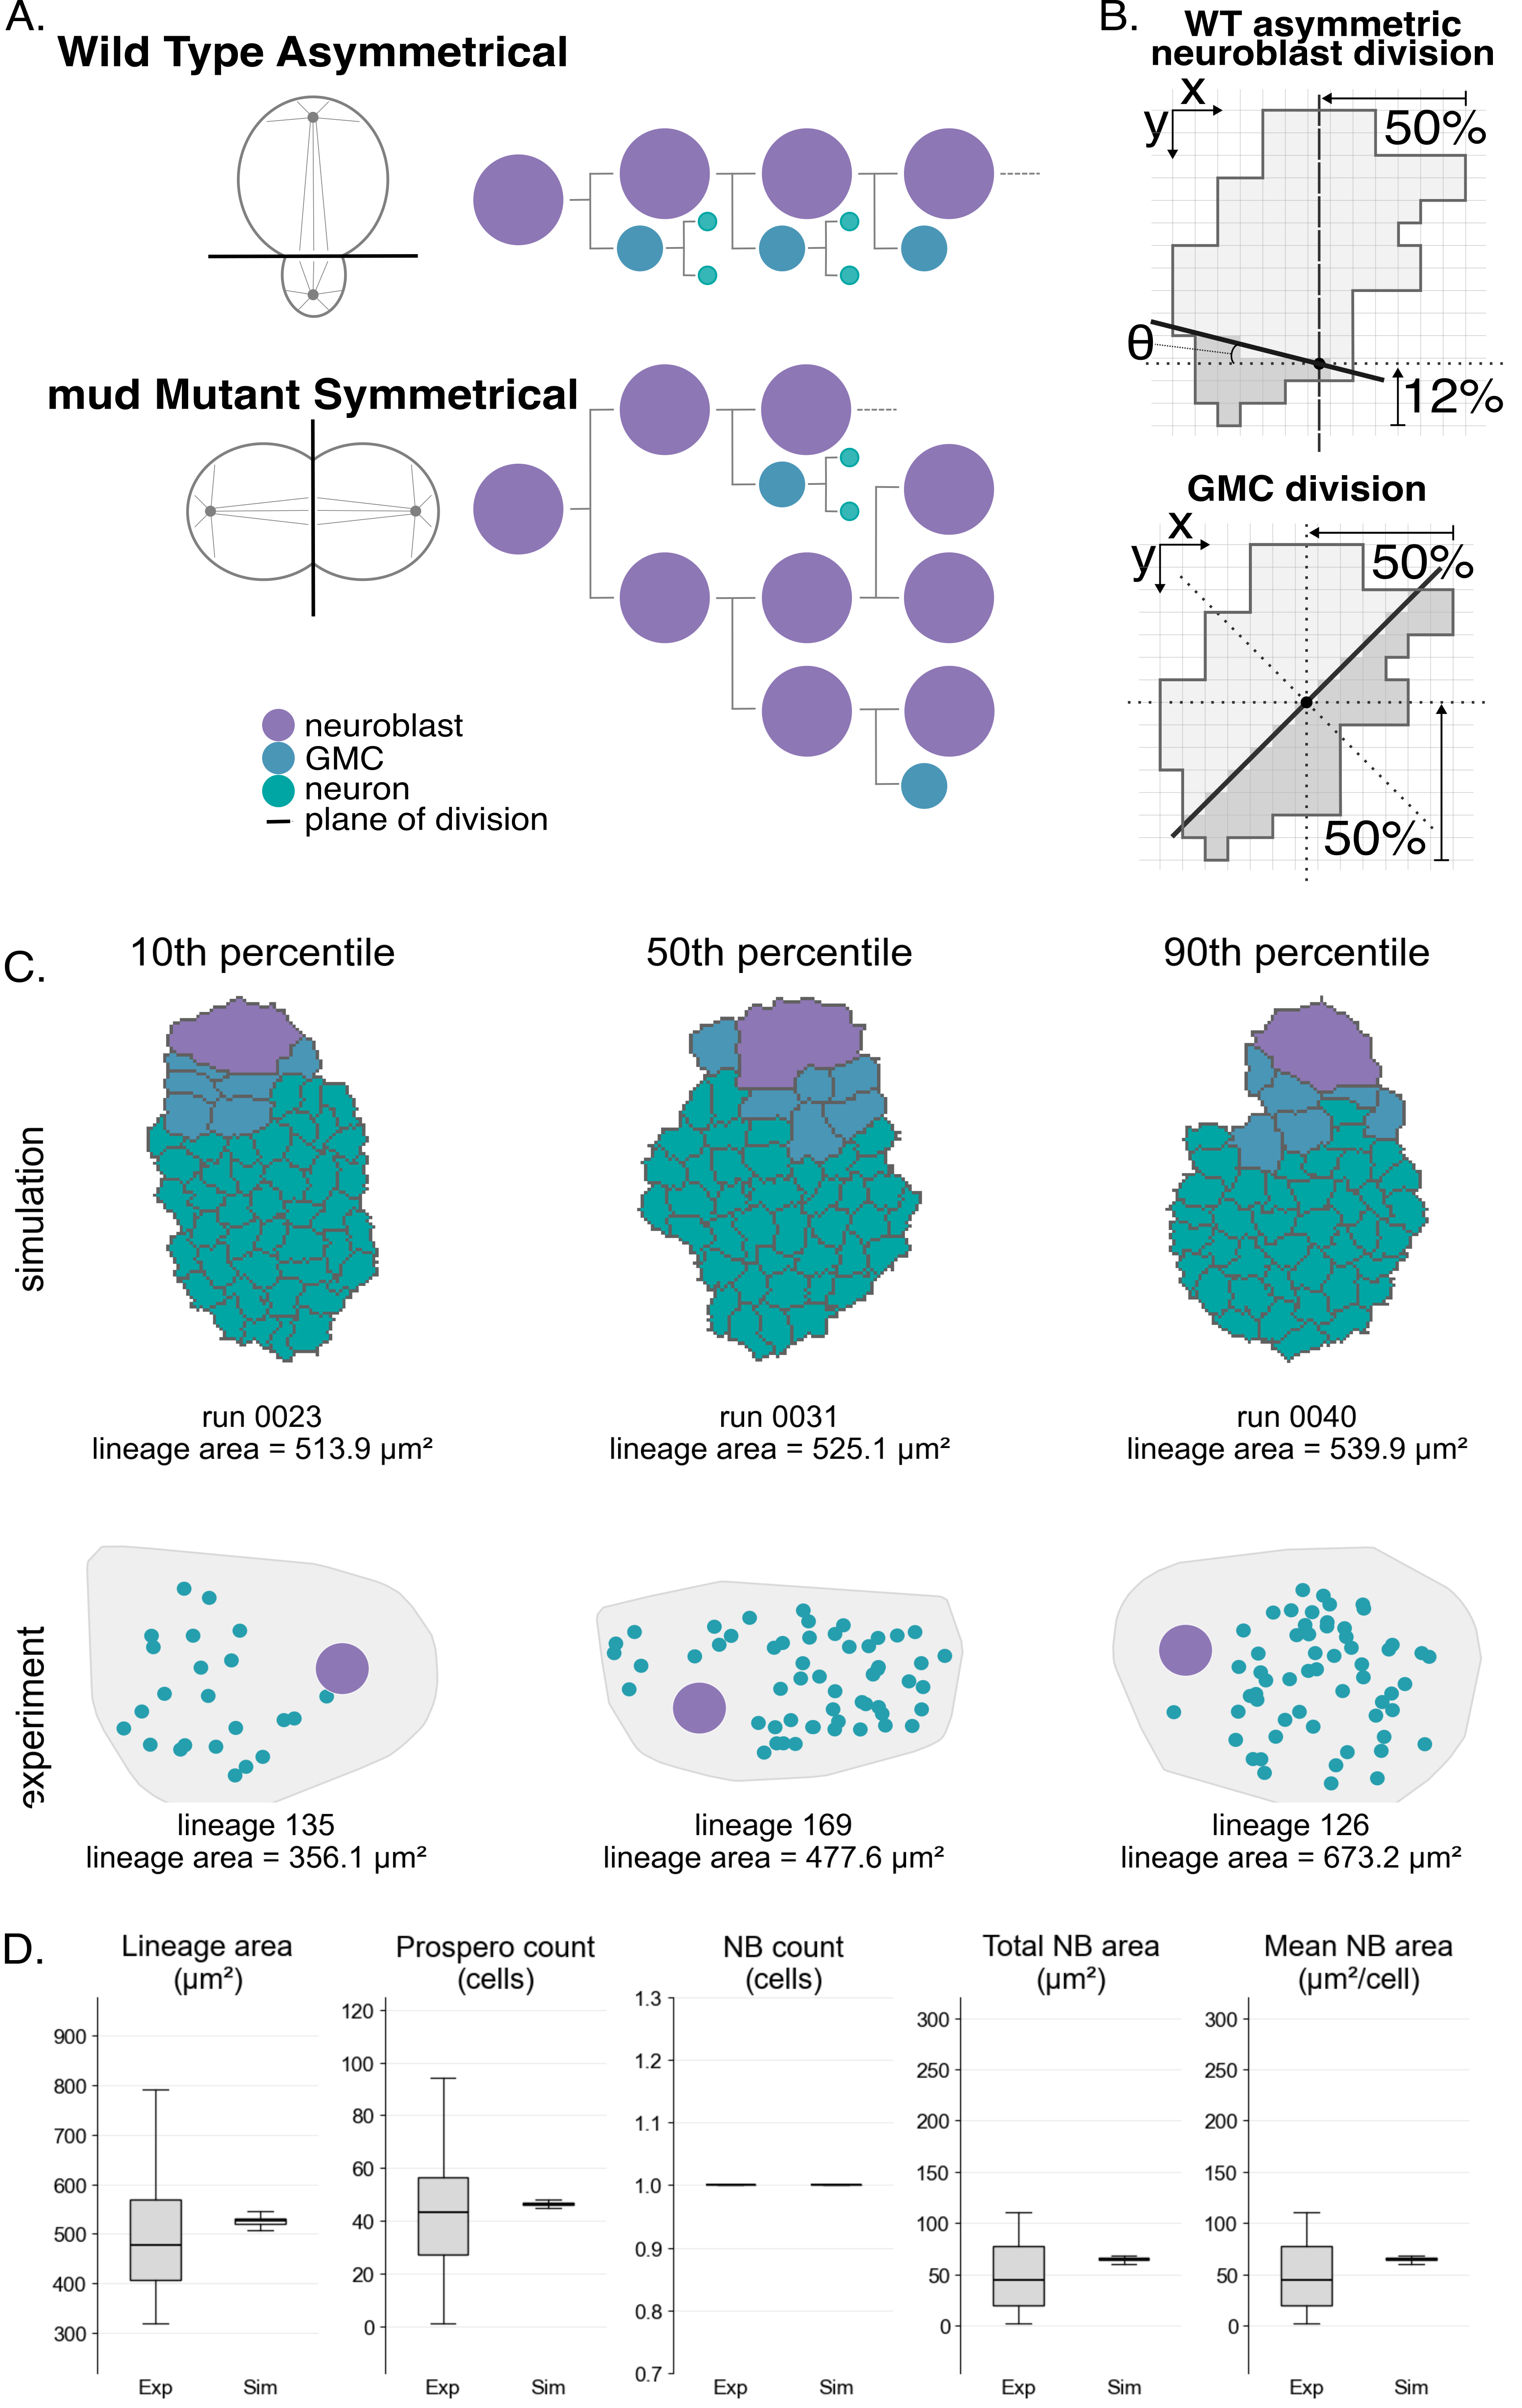
\includegraphics[width=.75\textwidth]{fig1/fig1.png}
\caption{\textbf{Calibrated CPM of developing neuroblast lineage recapitulates expected WT lineage scale, composition, and organization.} 
A. WT and mud Mutant planes of division and differentiation cascades.
B. Schematic of how the CPM implements asymmetric division and GMC division.
C. Top: Three example simulated WT neuroblast lineages reflecting the 10th, 50th and 90th percentile of lineage area across all WT simulations. Bottom: The distribution of cells in three experimentally imaged WT lineages. Dots represent nuclear centroids.
D. Distributions of five calibration metrics across experimental and simulated lineages.}
\label{ch3-fig1}
\end{figure}

To establish a baseline WT model for later perturbation analyses, we first calibrated a spatiotemporal CPM-based ABM of the developing \textit{Drosophila} neuroblast lineage.
In the WT rule set, the neuroblast divides after growing to $1.166\times$ its initial size.
Each neuroblast has an apical axis (Figure \ref{ch3-fig1}B dashed line) and a default plane of division which passes through a point located $88\%$ down the apical axis from the apical end of the cell and centered laterally (Figure \ref{ch3-fig1}B top dashed line).
By default, that division plane is perpendicular to the apical axis (Figure \ref{ch3-fig1}B top dashed line), and division-to-division angular variation is sampled from a distribution centered at $0^\circ$ with a standard deviation of $26^\circ$, matching the scale of the experimental WT angle distribution (see supplemental figure).
Following division, the larger apical daughter remains a neuroblast, whereas the smaller basal daughter becomes a ganglion mother cell (GMC).
The GMC then undergoes one final symmetric division along the cardinal axis that yields the longest new cell membrane (Figure \ref{ch3-fig1}B bottom) to produce two neurons. 
Neurons neither grow nor divide.
Full parameter values and the calibration workflow are described in Methods.
% Parameterization details to port into Methods from ARCADE/PARAMETERS_EXPLAINED.md.

We anchored this calibration to WT endpoint summaries derived from the experimental dataset in \texttt{data/exp/processed/exp\_summary.csv}.
See Methods for experimental data preprocessing details.
In that dataset, WT lineages contained a mean of $44.93 \pm 21.68$ Pros$^{+}$ cells and exactly one Dpn$^{+}$ neuroblast at the terminal time point.
WT lineage area averaged $501.2 \pm 125.8~\mu\mathrm{m}^2$, and because WT lineages end with one neuroblast, total and mean neuroblast area were both $51.9 \pm 42.6~\mu\mathrm{m}^2$.
We calibrated the baseline WT condition shown here (\texttt{wt\_divMean0Stdev26}, \texttt{sim61}, \texttt{VCV=1}) to match these five metric summaries.
Across simulated WT runs, the model produces lineages with a mean area of $525.4~\mu\mathrm{m}^2$, $46.42$ Pros$^{+}$ cells, one Dpn$^{+}$ neuroblast, and a mean neuroblast area of $64.2~\mu\mathrm{m}^2$, placing the simulated distribution within one standard deviation of the experimental WT mean for all calibration targets (Figure\ref{ch3-fig1}D).

Representative simulated WT lineages also qualitatively resemble experimental WT lineages across the observed range of lineage sizes (Figure\ref{ch3-fig1}C).
In both simulation and experiment, the neuroblast typically remains peripheral to the lineage while differentiated GMCs and neurons occupy most of the interior.
Importantly, this peripheral organization was not itself a calibration target.
Instead, the calibration is performed only against endpoint lineage scale and composition, allowing the spatial organization used in later sections to function as an emergent model behavior rather than a quantity fit by construction.

Together, these results indicate that the calibrated WT CPM captures the expected scale and composition of the lineage while remaining sufficiently unconstrained spatially to serve as a mechanistic testbed for hypotheses about division geometry and lineage organization.

\subsection{Distinct components of WT division geometry differentially affect lineage organization.}

Because spatial organization emerged in the calibrated WT model without being used as a fitting target, we next used that baseline to test which aspects of the imposed division geometry were most important for maintaining the sorted WT lineage morphology.
In the model, WT division dynamics contain three separable geometric components.
These are the orientation of the apical axis, the amount of rotation applied to the default plane of division, and the degree to which the division plane is offset away from the apical membrane.
We systematically perturbed each component while holding the others constant in order to assess its impact on lineage organization.
To quantify those effects, we used two spatial readouts.
First, we measured normalized heterotypic contact fraction, which reports the extent to which neuroblast and non-neuroblast cell territories intermingle relative to the amount of mixing expected from the lineage composition alone (see Methods).
Second, we measured the fraction of the neuroblast perimeter exposed to extracellular space, which reports how peripherally the neuroblast remains positioned within the lineage.
Together, these metrics distinguish lineages in which the neuroblast remains spatially segregated at the edge from lineages in which it becomes internalized and more intermixed with differentiated progeny.

\begin{figure}[!htbp]
\centering
\vspace{-1.5cm}
\includegraphics[width=.95\textwidth]{fig2/fig2.png}
\caption{\textbf{Impact of decoupled components of WT division geometry on lineage organization.} 
A. Depictions of intergenerational rotation mean shift (top), fixed-axis variance sweep (bottom left), and offset shift (bottom right) mechanisms implemented to decouple apical axis orientation, stochastic rotation, and offset shift in the CPM.
B. Distribution of normalised heterotypic contact values (top) and NB perimeter fraction values (bottom) across different simulated conditions.
C. Example lineages drawn from each of the simulated conditions. }
\label{ch3-fig2}
\end{figure}

\subsubsection{Persistent intergenerational rotation disrupts WT lineage sorting.}
To test the contribution of persistent intergenerational reorientation, we first varied the amount by which the apical axis rotated from one division to the next (\ref{ch3-fig2} A top).
In these simulations, fixed-axis variance is held at the biologically grounded WT value of $26^\circ$, and the division offset is held at the calibrated WT value of $88\%$.
The baseline WT condition uses no persistent mean-shift in intergenerational orientation, whereas perturbed conditions impose apical-axis reorientation drawn from distributions centered at $45^\circ$ or $90^\circ$.

Introducing persistent intergenerational rotation causes a marked loss of the sorted WT morphology (\ref{ch3-fig2} B left, C top).
Relative to the baseline WT condition, lineages with imposed reorientation show substantially higher normalized heterotypic contact and reduced neuroblast exposure to extracellular space, consistent with neuroblast internalization and increased mixing among cell types.
This effect is clear at $45^\circ$ and remains strong at $90^\circ$.
Thus, within the model, maintaining a stable relative orientation across generations appears to be an important requirement for preserving the peripheral neuroblast position and the spatially sorted architecture of the developing WT lineage.

\subsubsection{Increasing fixed-axis variance has limited effects until extreme values.}
We next asked whether increasing stochastic variation around a stable WT division axis was sufficient to disrupt lineage organization.
To isolate this effect, we returned the intergenerational rotation mean to the baseline WT value of $0^\circ$ and held the division offset at $88\%$.
We then increased the standard deviation of fixed-axis variation from the biologically grounded WT value of $26^\circ$ through progressively broader distributions (\ref{ch3-fig2} A bottom left).
This perturbation differs conceptually from the persistent intergenerational rotation tested above.
Here, successive divisions continue to fluctuate around the same underlying orientation, rather than drifting persistently away from it over generations.

Across this variance sweep, moderate increases in fixed-axis variability produce only modest changes in lineage organization (\ref{ch3-fig2} B center, C center).
Normalized heterotypic contact rises gradually as the variance increases, but the effect remains substantially smaller than the disruption caused by persistent intergenerational rotation.
Likewise, neuroblast exposure to extracellular space declines progressively across the sweep rather than collapsing immediately.
Qualitatively, these lineages largely retain their sorted morphologies, with the neuroblast still positioned near the lineage periphery.
Thus, the calibrated WT lineage tolerated appreciable stochastic variation around a stable axis while largely preserving its sorted morphology.

At the highest tested variance ($90^\circ$), however, this tolerance begins to break down.
Under this extreme condition, large rotations of the default division axis produce more mixing and reduced neuroblast exposure.
Even so, the resulting disorganization remains weaker than that produced by persistent intergenerational rotation (\ref{ch3-fig2} B center, C center).
These results indicate that stochastic division-angle variability can disrupt lineage organization, but only when it becomes very large.
Within the model, these results suggest that preserving a consistent central orientation across generations is more important for maintaining WT spatial organization than tightly minimizing every division-to-division fluctuation around that orientation.

\subsubsection{Reducing asymmetric offset produces only modest disorganization relative to intergenerational rotation.}
We next asked how strongly lineage organization depends on maintaining the WT asymmetric division offset.
To isolate this effect, we held the intergenerational rotation mean at the baseline WT value of $0^\circ$ and the fixed-axis variance at $26^\circ$ while shifting the division plane progressively away from the calibrated WT offset of $88\%$ toward more symmetric placements (\ref{ch3-fig2} A bottom right).
We tested offsets of $75\%$, $62\%$, and $50\%$.

Moving the division plane toward the center increases both normalized heterotypic contact and neuroblast internalization, indicating a measurable loss of lineage sorting (\ref{ch3-fig2} B right, C bottom).
However, across this sweep, the magnitude of the effect remains smaller on average than that produced by persistent intergenerational rotation (\ref{ch3-fig2} B right).
Qualitatively, the offset-perturbed lineages also remain fairly organized, with the neuroblast still generally occupying a peripheral position even when it if fully surrounded by cells (\ref{ch3-fig2} C bottom).
Thus we conclude that although maintaining the WT offset contributes to robust sorting, the model does not suggest that offset alone is the dominant determinant of lineage organization.

One complication in interpreting this perturbation is that reducing the offset increases daughter birth sizes and therefore lineage size.
In the smaller simulation domains used initially, these larger lineages frequently encountered the domain boundaries.
We therefore repeated the offset-shift simulations in expanded fields of view, although even in those larger domains some lineages still contacted the walls at later times.
For that reason, we interpret the offset-shift results more cautiously than the intergenerational-rotation and fixed-axis-variance results.
Even with that caveat, both the quantitative spatial readouts and the representative lineages support the same qualitative conclusion: reducing asymmetric offset perturbs sorting, but less strongly than persistent intergenerational rotation.

\subsection{Cell-size effects are insufficient to constrain \textit{mud} mutant lineage overgrowth.}
We next used our model to explore which regulatory mechanisms would be sufficient to constrain lineage overgrowth in \textit{mud} mutants.
We implemented a \textit{mud} mutant cell type with the same baseline parameters as our calibrated WT simulations, then added a rule for symmetric division: whenever the division plane rotates past $45^\circ$ from the apical/basal axis, the cell deterministically divides symmetrically along that axis, yielding two neuroblast daughters.
Because division-plane rotation is drawn from a normal distribution with mean $0^\circ$ and standard deviation $26^\circ$, this rule causes \textit{mud} mutant neuroblasts to divide symmetrically about 13\% of the time.
Both this rate and the rotation-based trigger are consistent with experimental observations.
We also set the adhesion parameter so that neuroblasts would have stronger adhesion to each other than to all other cells to reflect the experimental observation that neuroblasts in \textit{mud} mutant lineages tend to be next to each other.

We first asked whether the cell-size difference between symmetrically and asymmetrically derived NBs was itself sufficient to constrain mutant lineage overgrowth.
Because symmetric division produces two undersized daughters, fixing the division-volume threshold at the value expected for WT NBs would force mutant NBs born of symmetric divisions to spend additional time growing before dividing again, slowing lineage expansion.
We therefore implemented a constant division threshold calibrated to the expected WT division volume (see Methods) and simulated \textit{mud} mutant lineages with all other parameters held at their WT values.

\begin{figure}[!htbp]
\centering
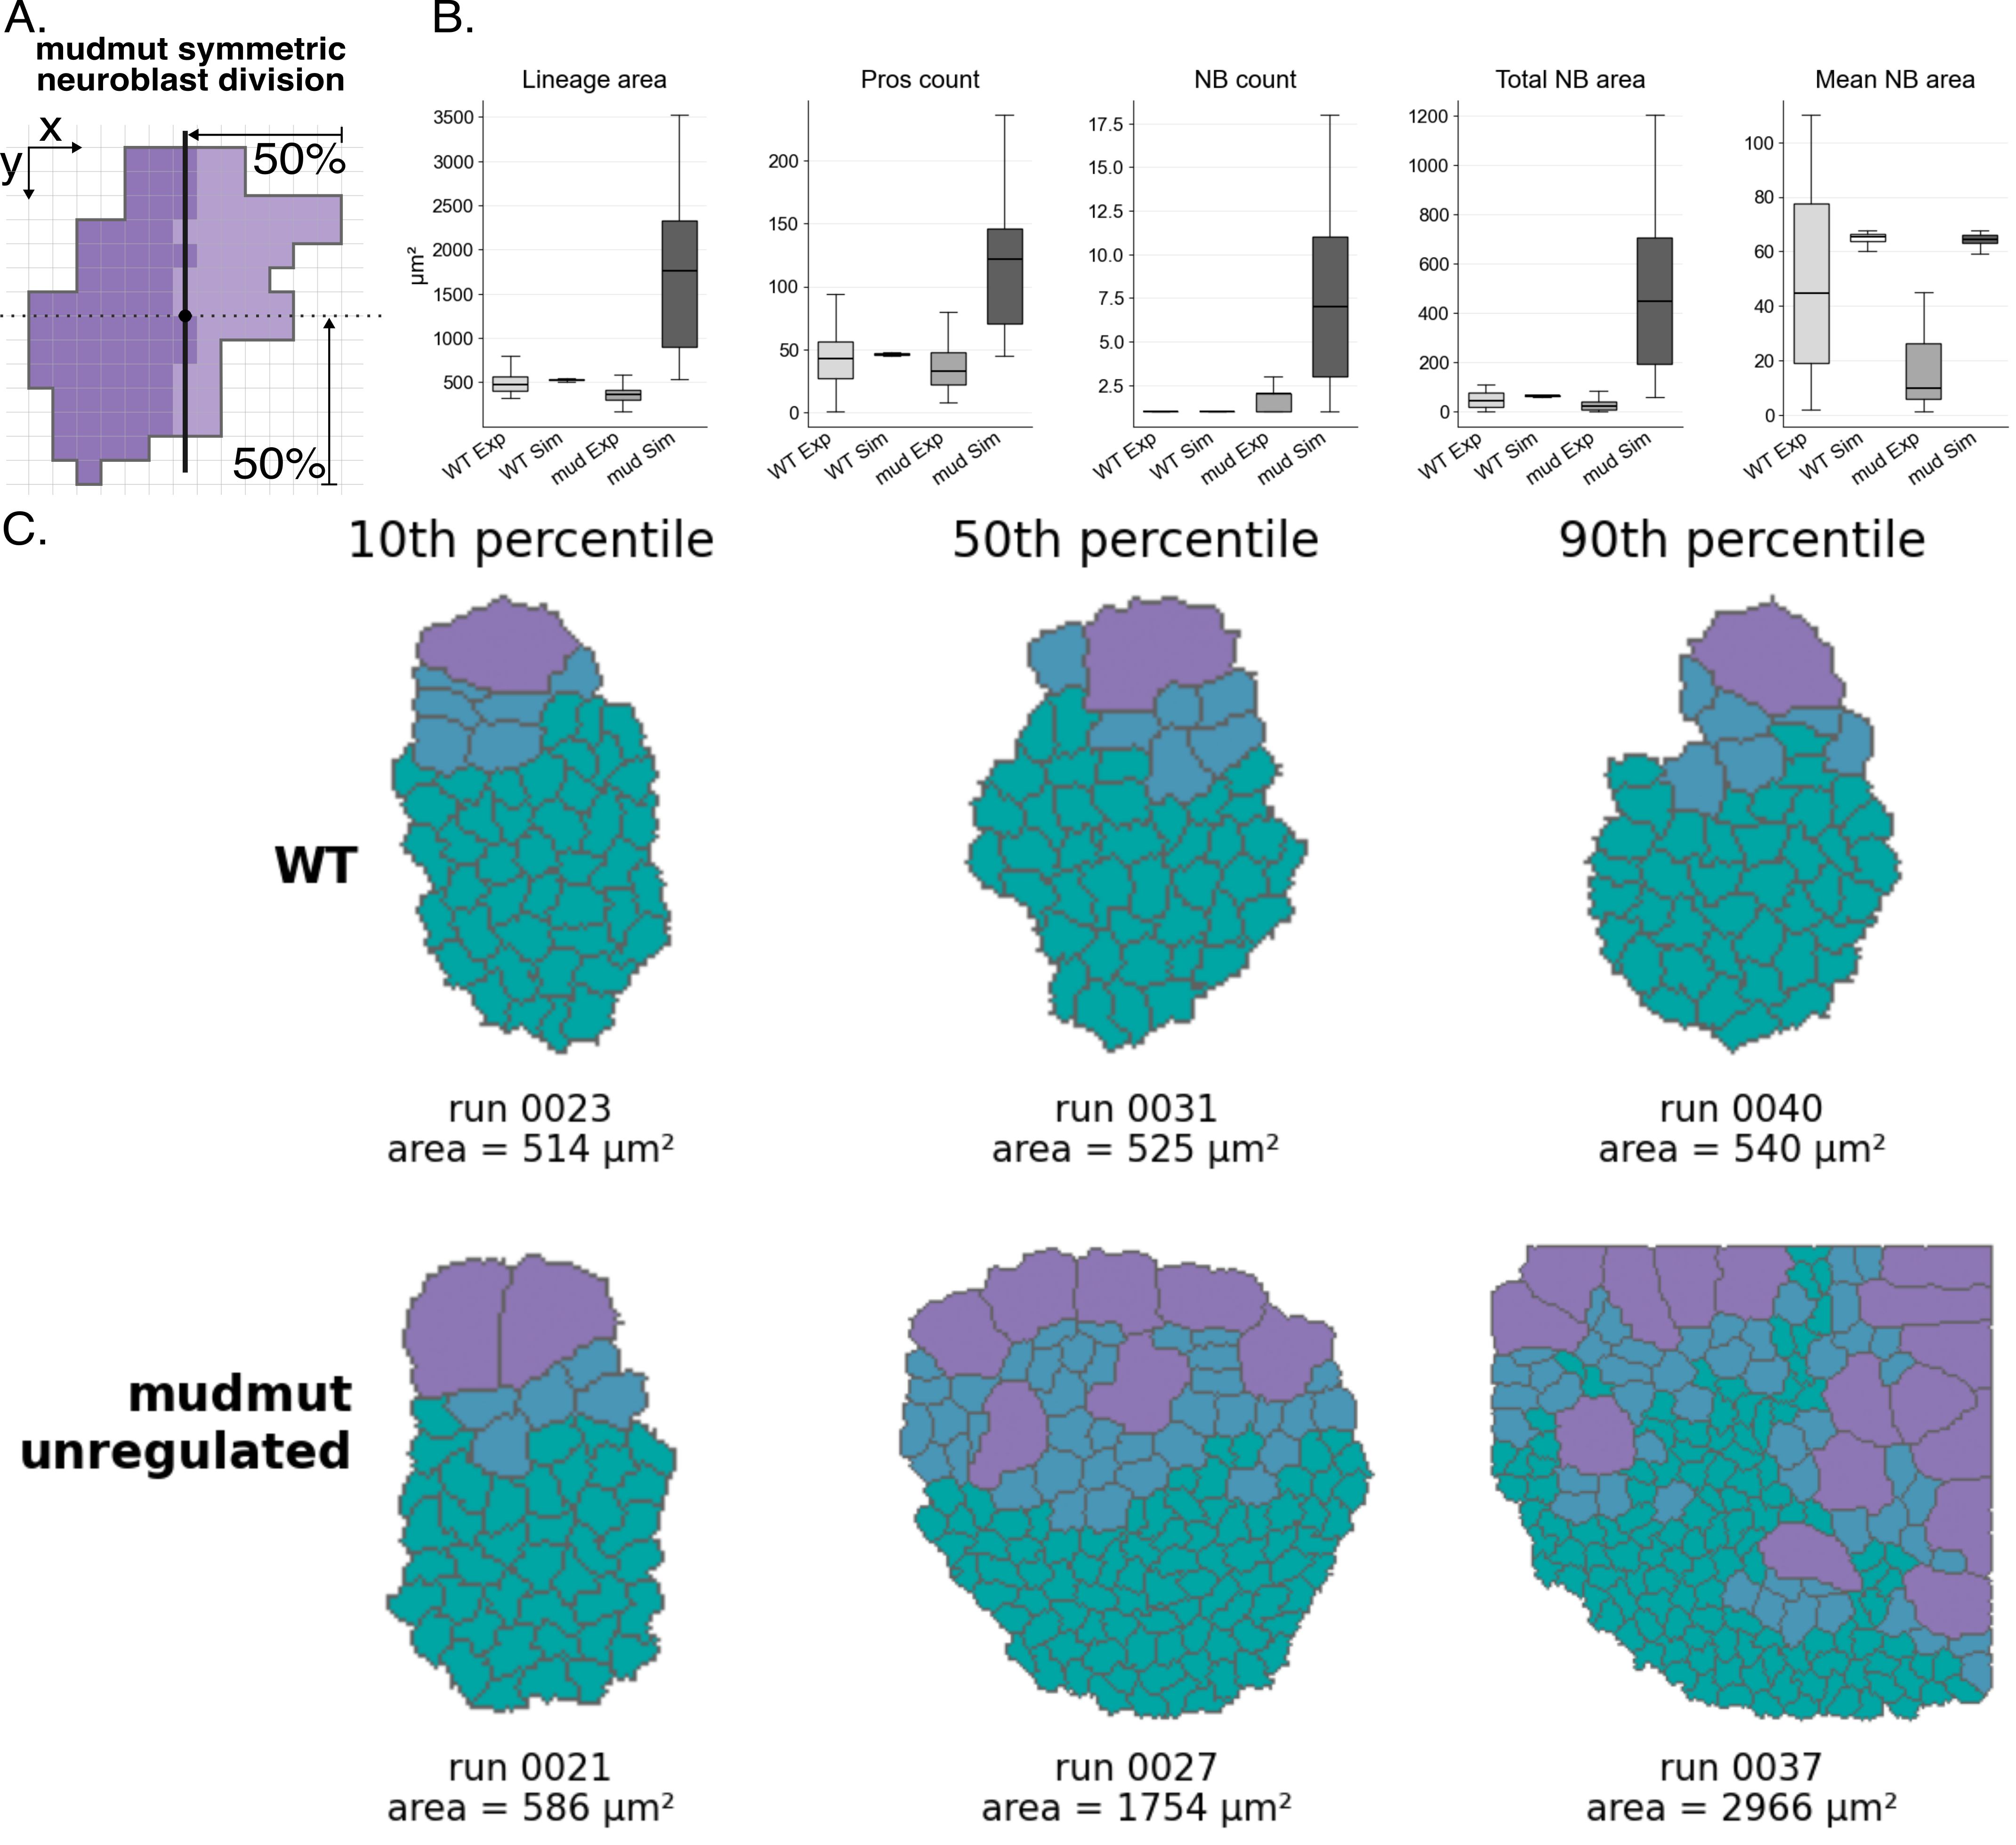
\includegraphics[width=.9\textwidth]{fig3/fig3.png}
\caption{\textbf{The model predicts that unregulated \textit{mud} mutant lineages should overgrow WT lineages.}
\textbf{A.} Schematic of an NB undergoing symmetric division as implemented in the model.
\textbf{B.} Distributions of five non-spatial calibration metrics across WT experimental, WT simulated, \textit{mud} mutant experimental, and unregulated \textit{mud} simulated lineages.
\textbf{C.} Representative WT and unregulated \textit{mud} mutant simulated lineages at the 10th, 50th, and 90th percentiles of lineage area.}
\label{ch3-fig3}
\end{figure}

The simulated \textit{mud} mutant lineages outgrew the simulated and experimental WT lineages by all five of our calibration metrics. %TODO: make sure I have consistent language around these metrics. "Calibration metrics"

\subsection{Candidate regulatory mechanisms constrain mud mutant overgrowth only when division thresholds scale with birth size.} %TODO: EDIT THIS SECTION

Two salient differences between \textit{mud} mutant and WT neuroblast lineages are that \textit{mud} mutant lineages have more NBss and that the NBs in \textit{mud} mutant lineages are on average smaller than WT neuroblasts (supplemental data).
We were curious whether regulation based on either of those features could constrain mutant lineage overgrowth.
To explore this, we implemented four regulatory regiemes.
In neuroblast volume based (VOL) regulation, we set a constant reference NB volume which is equal to the expected average volume of a WT NB.
NB growth rate is repressed if its volume is less than that reference and accelerated if its volume is greater than that reference point.
This is exploring the hypothetical scenerio in which growth rate is linked to neuroblast volume and asking whether, in this system, that regime would be sufficient to constrain mutant neuroblast lineage growth.
We implemented this regulation in both an ABM-like and PDE-like manner.
In the ABM-like implementation, each NB's growth rate is independently regulated by its volume.
In the PDE-like implementation, all NBs in the simulation have the same growth rate, and each NB's growth rate is regulated by the average volume across all NBs in the simulation.
The PDE-like implementation allows us to explore a hypothetical situation in which the growth rate of NBs is influenced by both the NB's own volume and the volume of the other NBs in the simulation.
We also implemented a NB-contact (NB) based regulation.
In this regieme, NB growth rate is suppressed via a hill function based on how many NB neighbors the NB has.
We similarly implemented this in both an ABM and PDE-like manner.
In the ABM-like implementation each NB's growth is repressed by its number of NB neighbors and in the PDE-like manner eahc NB's growth is repressed by the total number of NBs in the simulation.
This could represent some kind of diffusible signaling factor.

We applied both of these regulatory regiemes with both the constant division threshold (VCV=0) and a dynamic division threshold (VCV=1) in which the NB division volume threshold is a function of the starting NB volume Figure\ref{ch3-fig4} A.

We first confirmed that each of the four candidate regulatory dynamics, when applied to our calibrated WT cell type, leaves the five non-spatial calibration metrics broadly within the WT experimental range (supplement).

When simulated with the fixed division threshold (VCV=0), none of the four regulatory mechanisms, simulated \textit{mud} mutant lineages remained well above the experimental \textit{mud} range on lineage area, Pros count, NB count, and total NB area (Fig.~\ref{ch3-fig4}B, light boxes).
NB-contact regulation came closest of the four but did not bring all five calibration metrics into agreement with the experimental data.

\begin{figure}[!htbp]
\centering
\includegraphics[width=.9\textwidth]{fig4/fig4.png}
\caption{\textbf{Volume-based regulation paired with birth-size-dependent division thresholds constrains \textit{mud} mutant lineage overgrowth.}
\textbf{A.} Schematic contrasting the two threshold rules.
\textbf{B.} Endpoint distributions of the five calibration metrics across the unregulated baseline plus four candidate regulatory dynamics (NB-ABM, NB-PDE, volume-ABM, volume-PDE), under each threshold rule (light: VCV=0; dark: VCV=1). The red band marks the experimental \textit{mud} interquartile range; the dashed red line marks the experimental median. Y-axes are log-scaled.
\textbf{C.} Representative simulated \textit{mud} mutant lineages at the 50th percentile of lineage area, organized by regulatory dynamic (columns) and threshold rule (rows).}
\label{ch3-fig4}
\end{figure}

We then re-ran the same four candidate regulatory dynamics with VCV=1, the threshold rule under which each NB divides at a multiple of its own birth size rather than at a shared absolute volume.
The biological intuition is that, under this rule, the cell-size memory established by a symmetric division propagates forward across generations: a smaller-born mutant NB has a smaller division threshold, so it divides at a smaller volume, producing daughters that are themselves smaller still (Fig.~\ref{ch3-fig4}A).
This keeps \textit{mud} mutant NBs that originate from a symmetric division persistently deeper in the repressive regime imposed by the regulatory dynamic, rather than allowing them to recover to WT-equivalent volumes after a single cycle.

Under this threshold rule, the volume-based regulatory dynamics brought simulated \textit{mud} mutant lineages into the experimental range on lineage area, Pros count, NB count, and total NB area (Fig.~\ref{ch3-fig4}B, dark boxes; Fig.~\ref{ch3-fig4}C,D).
Mean NB area is the one metric on which volume-PDE drifts below the experimental range: the smaller per-cycle thresholds produce smaller individual NBs, undershooting the experimental average. %TODO: confirm consistency with biological expectations or note as caveat.
NB-contact regulation under VCV=1 also tracks the experimental range more closely than it did under VCV=0, but remains less precise than the volume-based dynamics across the calibration metrics.
The missing ingredient in the unregulated and VCV=0-regulated cases was therefore not a different regulatory mechanism, but a different threshold rule.

Together, these results indicate that constraining \textit{mud} mutant lineage overgrowth in our model requires both a regulatory dynamic that responds to local cellular context and a threshold rule that allows the smaller birth size of symmetric-division descendants to propagate forward in time.

\subsection{Preferential NB–NB adhesion is not required for NB clustering in regulated \textit{mud} mutant lineages}

In the simulated \textit{mud} mutant lineages from Result 4, neuroblasts frequently appeared adjacent to one another, particularly under the volume-based regulatory dynamics that brought lineages closest to the experimental \textit{mud} range.
We had initialized these simulations with preferential NB–NB adhesion so we asked whether this adhesion term was responsible for the observed clustering.

We re-ran the volume-based simulations under VCV=1, this time setting the NB–NB adhesion strength equal to all other cell-cell adhesions in the simulation, and compared each run to its with-adhesion counterpart at the same seed.

Removing preferential NB–NB adhesion produced nearly indistinguishable distributions on two of the three spatial metrics: the normalized heterotypic contact fraction, a measure of mixing between NBs and non-NB progeny (Fig.~\ref{ch3-fig5}B), and the homotypic NB contact fraction, the fraction of NB inter-cell contacts that are NB-to-NB (Fig.~\ref{ch3-fig5}D).
Both volume-based regulatory dynamics retained roughly 20\% of NB inter-cell contacts as NB-NB regardless of adhesion state, indicating that NB clustering in this model emerges from birth geometry and limited subsequent displacement rather than from a preferential adhesion term.
Representative paired lineages confirmed this visually (Fig.~\ref{ch3-fig5}A): the spatial layout of NBs and progeny looks essentially the same with or without preferential adhesion.

%The one metric that did differ modestly between adhesion states was the fraction of NB perimeter exposed to extracellular space (Fig.~\ref{ch3-fig5}C), which shifted slightly and in opposite directions for the two regulatory dynamics.
%We interpret this as evidence that preferential adhesion can affect how NBs are positioned at the lineage surface, but does not affect either the mixing of NBs with progeny or the homotypic clustering of NBs themselves.

\begin{figure}[!htbp]
\centering

\includegraphics[width=.7\textwidth]{fig5/fig5.png}
\caption{\textbf{Removing preferential NB-NB adhesion has minimal effect on NB clustering or mixing in regulated \textit{mud} mutant lineages.}
\textbf{A.} Representative simulated \textit{mud} mutant lineages from each (regulatory dynamic $\times$ adhesion state) combination, picked closest to the mean homotypic NB contact fraction within their group. Rows: regulatory dynamic (volume-ABM, volume-PDE under VCV=1). Columns: with vs without preferential NB-NB adhesion.
\textbf{B.} Distributions of the normalized heterotypic contact fraction (a measure of mixing between NBs and non-NB progeny) for each regulatory dynamic, the fraction of NB perimeter exposed to extracellular space, and the fraction of NB inter-cell contacts that are NB-to-NB, with and without preferential NB-NB adhesion.}
\label{ch3-fig5}
\end{figure}

Together, these results indicate that the NB proximity observed in our model is largely a consequence of birth geometry and limited divisions in constrained mutant lineages and does not require an adhesion-driven mechanism to be maintained.

\input{_discussion.tex}
\input{_conclusion.tex}
\section{Methods}

\subsection{Immunohistochemistry}
Primary antibodies used in this study were rat anti-dpn (1:100, Abcam 11D1BC7), mouse anti-pros (1:500, gift from Chris Doe)

Secondary antibodies used were goat anti-rat (AlexaFluor 647, Invitrogen A21247), goat anti-mouse (AlexaFluor 405, Invitrogen A31553), goat anti-rabbit (AlexaFluor 405, Invitrogen A31556), goat anti-rabbit (AlexaFluor 647, Invitrogen A21245). All secondary antibodies were used at 1:1000. All experiments were conducted with at least 1 overnight in primary and 1 overnight in secondary antibody.

Larvae were dissected by removing the posterior half and inverting, then removing organs, and severing the connections between the back end of the brain and the mouth parts, to minimize stretching of the brain during fixation.
Dissected larvae were put in schneiders insect media until fixation. Fixation was performed in 4\% PFA in schneiders medium on a nutator for 20 minutes.
PFA was then washed off with PBSBT (PBS, 1\% BSA, 0.1\% Triton-X) 3 times for 20 minutes on a nutator at room temperature.
Antibodies were diluted in PBSBT and samples were incubated on a nutator at 4C. After primary staining, samples were washed with PBSBT 3 times for 20 minutes on a nutator at room temperature.
Secondary antibody, also diluted in PBSBT, was then applied and incubated on a nutator at 4C.
After secondary staining, samples were again washed 3 times for 20 minutes on a nutator at room temperature.
Brains were then dissected off of the cuticles and put into vectashield.
Brains were mounted on glass slides in a small channel of vectashield between two spacers (glass coverslips), with a third coverslip on top.
All samples were imaged immediately after mounting on slides.

\subsection{Immunohistochemistry image segmentation and analysis}

To quantify Dpn volume, lineage volume, Pros+ cell number and Dpn number/lineage, we used Imaris 9.6 (and higher) to segment Dpn+ and Pros+ nuclei. Similarly, lineages were segmented and manually corrected if necessary. For lineage volume quantification, axonal projections were manually cut to account for image depth variations in our datasets. Segmentation was done by training Imaris’ pixel classifier or by using threshold segmentation.

\subsection{Experimental lineage dataset and preprocessing}

Experimental lineage measurements were derived from three-dimensional microscopy segmentations of \textit{Drosophila} larval brain lobes.
For each lobe, three VRML (\texttt{.wrl}) files were available: lineage hull segmentations, Dpn-positive nuclei, and Pros-positive nuclei.
The analyzed dataset included WT control lobes (\texttt{lobe1}, \texttt{lobe2}, \texttt{lobe7}, \texttt{lobe8}, \texttt{lobe13}, and \texttt{lobe15}), \textit{mud} mutant lobes (\texttt{lobe110}, \texttt{lobe113}, \texttt{lobe116}, and \texttt{lobe119}), and nanobody perturbation lobes (\texttt{lobe16}, \texttt{lobe17}, \texttt{lobe19}, \texttt{lobe20}, \texttt{lobe21}, and \texttt{lobe22}).

Experimental preprocessing uses the local pipeline implemented in LINK TO REPO WITH \texttt{scripts/preprocess\_exp.py} and \texttt{src/npa/exp\_preprocessing/}.
WRL files are parsed into triangle meshes by extracting vertex and face blocks from the VRML text and fan-triangulating polygonal faces.
Pros-positive cells are assigned to lineage hulls by bounding-box overlap, with assignment requiring at least $95\%$ of vertices to fall within a lineage bounding box.
Dpn-positive cells are assigned by sampled mesh containment, using a bounding-box prefilter followed by containment testing of 20 sampled vertices and requiring at least $60\%$ of sampled vertices to lie within a lineage hull.

Lineages are excluded before analysis if they fail either of two quality-control criteria.
First, lineages are rejected as disconnected if they contain a secondary connected component with at least 50 faces and volume at least 5.0 in the native WRL coordinate system.
Second, lineages are rejected if no Dpn-positive cell can be assigned to the lineage.
Rejected lineages are preserved in a separate index but are excluded from all summary analyses.
Among WT lineages, 60 of 143 total segmented lineages were retained after filtering (2 lineages were rejected as disconnected and 81 rejected for lacking an assigned Dpn-positive cell).
Among \textit{mud} mutant lineages, 59 of 63 total segmented lineages were retained after filtering, and the retained lineages included between 1 and 5 Dpn-positive cells.

For each retained lineage, the lineage hull vertices are projected into two dimensions using the first two principal components of the three-dimensional hull geometry.
The projected lineage outline is represented by the convex hull of the projected vertices, buffered by $0.5 \times ds$ with \(ds = 0.3~\mu\mathrm{m}\).
To generate analysis tensors aligned with the simulation outputs, each projected lineage is rasterized onto a \(200 \times 200\) canvas.
Pixels inside the lineage hull are assigned to the nearest Dpn or Pros centroid using a Voronoi tessellation, yielding a two-channel tensor in which channel 0 represents Dpn territory and channel 1 represents Pros territory.
Per-lineage mesh files and stacked genotype-level analysis tensors are written to \texttt{data/exp/processed/}.

Experimental endpoint summaries are then computed from the processed lineage dataset.
For each lineage we recorded the number of Dpn-positive cells (\texttt{n\_dpn}), the number of Pros-positive cells (\texttt{n\_pros}), lineage area in occupied pixels (\texttt{lin\_area\_vox}), total Dpn area (\texttt{dpn\_area\_vox}), and mean Dpn area per lineage (\texttt{avg\_dpn\_area\_vox}).
Genotype-level means and standard deviations are written to \texttt{data/exp/processed/exp\_summary.csv} and used as the experimental reference for model calibration and comparison.

\subsection{Cellular Potts model of WT and \textit{mud} mutant lineages}

All code for this model is publicly available at this url: ARCADE-URL.
All code for the analysis run in this manuscript is available at this url: REPO-URL.

We model neuroblast lineage development with a two-dimensional spatiotemporal Cellular Potts model implemented in the ABM framework ARCADE.
Although the simulations are visualized and analyzed in two dimensions, ARCADE uses a three-dimensional volume formalism, so growth and division thresholds are specified in \(\mu\mathrm{m}^3\) and represented on a lattice of height one voxel.
Unless otherwise noted, simulations run for 2161 ticks with \(dt = 0.01667\) h per tick, corresponding to 36 h of total biological time with 1 minute per tick.
The default lattice size is \(200 \times 200 \times 1\) voxels, with \(ds = 0.3~\mu\mathrm{m}\) per voxel edge.

\subsection{Cellular Potts Hamiltonian}

In a Cellular Potts model, each lattice site \(i\) is assigned a cell identity \(\sigma_i\), and each identity belongs to a cell type \(\tau(\sigma_i)\).
Cell morphology and movement emerge from stochastic updates that consider whether a given lattice site should take its neighbor's identity.
Whether a proposed copy is accepted depends on the resulting change in the Hamiltonian energy.

The full Hamiltonian can be written generically as
\[
H = H_{\mathrm{adhesion}} + H_{\mathrm{volume}} + H_{\mathrm{surface}}.
\]
The adhesion term is
\[
H_{\mathrm{adhesion}} = \sum_{\langle i,j \rangle} J\!\left(\tau(\sigma_i),\tau(\sigma_j)\right)\left(1-\delta_{\sigma_i,\sigma_j}\right),
\]
where \(\langle i,j \rangle\) indexes neighboring lattice sites, \(\sigma\) is the occupying cell identity or extracellular medium, \(\tau\) is the corresponding cell type, \(J\) is the contact-energy coefficient, and \(\delta_{\sigma_i,\sigma_j}\) is the Kronecker delta.
This term contributes only at interfaces between distinct cells or between a cell and extracellular space.

The volume constraint term is
\[
H_{\mathrm{volume}} = \sum_{\sigma} \lambda_v \left(v(\sigma)-V(\sigma)\right)^2,
\]
where \(v(\sigma)\) is the current cell volume, \(V(\sigma)\) is the target cell volume, and \(\lambda_v\) sets the strength of the volume penalty.
The surface constraint term is
\[
H_{\mathrm{surface}} = \sum_{\sigma} \lambda_s \left(s(\sigma)-S(\sigma)\right)^2,
\]
where \(s(\sigma)\) is the current cell perimeter, \(S(\sigma)\) is the target perimeter, and \(\lambda_s\) sets the strength of the surface penalty.

Proposed lattice updates are accepted according to the standard Metropolis rule
\[
P(\mathrm{accept}) =
\begin{cases}
1, & \Delta H < 0, \\
e^{-\Delta H/T}, & \Delta H \geq 0,
\end{cases}
\]
where \(\Delta H\) is the change in Hamiltonian associated with the proposed copy event and \(T\) is the simulation temperature.

In the simulations analyzed here, the contact-energy coefficient for cell--extracellular-space interfaces is 80, whereas the default cell--cell coefficient is 50.
Because lower contact-energy values correspond to stronger effective adhesion in this formalism, this choice ensured cohesion within each lineage, and prevented cells from dispersing into extracellular space.
For mutant simulations that included preferential NB adhesion, the NB--NB contact-energy coefficient was reduced further to 40.
Surface lambda values are 0.5 for neuroblasts, 1 for GMCs, and 2 for neurons.
Because the contribution of the surface term increases with cell size, these values are chosen so that cells of different types nevertheless maintain comparably smooth and rounded morphologies.
The Boltzmann temperature is visually calibrated to 18 so that WT neuroblasts can relax toward rounder shapes between successive asymmetric divisions.
Apoptosis is not included.

\subsection{WT growth and division rules}

In the WT rule set, the neuroblast grows until it reaches a division threshold equal to $1.166\times$ its initial volume and then divides asymmetrically.
The default WT division plane is perpendicular to the apical axis and passes through a point located \(88\%\) of the cell length from the apical edge and \(50\%\) across the lateral axis.
Default angular variation around the default division plane is drawn from a normal distribution centered at \(0^\circ\) with standard deviation \(26^\circ\).
This was based on the evaluation of experimental data that tracked the angle of cell divisions of WT NBs after each successive division (supplemental figure).
After WT division, the larger apical daughter remains a neuroblast and the smaller basal daughter becomes a GMC.
The GMC divides once more symmetrically to produce two neurons, and neurons neither grow nor divide.

\subsection{\textit{mud} mutant growth and division rules}
To model \textit{mud} mutant lineages, division-plane rotation at each division is drawn from a normal distribution centered at \(0^\circ\) with standard deviation \(50^\circ\), compared with \(26^\circ\) for WT.
We impose a threshold at \(\pm 75^\circ\) such that any sampled rotation exceeding \(75^\circ\) in magnitude is converted into a deterministic symmetric division along the neuroblast apical axis.
In the mutant rule set used here, this yields approximately 13\% symmetric divisions, consistent with experimental observation \cite{cabernard_2009_apicalbasalspindlea}.
Mutant daughter neuroblasts inherit apical axes rotated relative to the parent axis by an amount drawn from a normal distribution with mean \(0^\circ\) and standard deviation \(30^\circ\).
This inheritance rule is chosen to approximate the qualitative loss of stable spindle orientation observed experimentally in \textit{mud} mutant lineages.

\paragraph{Calibration of division-plane rotation parameters.}
The division-plane rotation standard deviation and symmetric-division threshold for \textit{mud} mutant simulations were calibrated from time-lapse measurements of NB division-axis angles tracked across successive divisions in \textit{mud} mutant and WT animals (Supplemental Figure X; see also \cite{cabernard_2009_apicalbasalspindlea}).
Step-to-step absolute rotation angles were computed from the change in the three-dimensional spindle-axis vector between consecutive time points and binned in \(15^\circ\) increments spanning \(0^\circ\)--\(180^\circ\).
The \textit{mud} mutant distribution contained no observed divisions in the \(75^\circ\)--\(90^\circ\) bin, whereas the WT distribution showed no analogous gap.
A similar discontinuity in \textit{mud} mutant division-axis rotation was reported by \cite{cabernard_2009_apicalbasalspindlea}.
We therefore set the symmetric-division threshold at \(75^\circ\): any rotation exceeding this value is classified as a symmetric division.

Under this threshold, \(13\%\) of observed \textit{mud} mutant division steps exceeded \(90^\circ\) and were classified as symmetric divisions, consistent with the symmetric-division frequency reported by \cite{cabernard_2009_apicalbasalspindlea}.
We calibrated the rotation standard deviation by finding the \(\sigma\) of a \(N(0,\,\sigma^2)\) distribution satisfying \(P(|X| > 75^\circ) \approx 13\%\), which yields \(\sigma = 50^\circ\).
As a cross-check, the empirical standard deviation of the observed step-to-step rotations computed after excluding values greater than \(90^\circ\) was \(44^\circ\), which we considered sufficiently consistent with the model value of \(50^\circ\).

\subsubsection{Imposed and volume-sensitive division thresholds}
The division threshold for \textit{mud} mutants is implemented in two different ways.
Under the fixed-threshold ruleset (\texttt{VCV=0}), all neuroblasts of a given type share the same critical volume \(V_c\), and division occurs when the cell reaches
\[
V \geq \mathrm{SIZE\_TARGET}\times V_c.
\]
In practice, this means \textit{mud} mutant cells divide when they surpass the same absolute threshold, which is set to \(1.166\times\) the expected WT neuroblast initial volume.

Under the birth-volume-dependent ruleset (\texttt{VCV=1}), daughter critical volume is reset from daughter birth volume.
For daughter neuroblasts, the new critical volume is
\[
V_{c,\mathrm{daughter}} = \max\!\left(V_{\mathrm{birth}},\,0.2V_{c,\mathrm{WT}}\right),
\]
where \(V_{c,\mathrm{WT}}\) is the baseline WT neuroblast critical volume.
For GMC daughters, the analogous rule is
\[
V_{c,\mathrm{GMC}} = \max\!\left(V_{\mathrm{birth}},\,0.1V_{\mathrm{NB,birth}}\right).
\]
Under this ruleset, the division threshold decreases as mutant daughter cells are born progressively smaller after successive symmetric divisions, but it cannot fall below a fixed minimum of \(20\%\) of the WT neuroblast critical volume (or \(10\%\) the initial GMC critical volume for the GMCs).
Biologically, this corresponds to the assumption that a cell can only divide if it remains above a minimum size.
Thus, \texttt{VCV=0} tests a fixed-threshold sizer hypothesis, whereas \texttt{VCV=1} allows daughter birth size to propagate into the next division threshold.

\subsubsection{NB growth regulatory mechanisms}
To test candidate mechanisms constraining mutant lineage growth, we vary whether neuroblast growth rate is regulated by cell volume or by NB--NB contact.
Each candidate repression mechanism can operate either in a cell-autonomous ABM-like mode or in a population-averaged PDE-like mode.

\paragraph{Volume-regulated growth.}
When volume-sensitive growth is enabled, the effective growth rate is scaled as a power law of cell volume relative to a reference volume.
In the ABM-like implementation, each cell updates its own growth rate according to
\[
r_i = r_0\left(\frac{V_i}{V_{\mathrm{ref}}}\right)^s,
\]
where \(r_0\) is the baseline growth rate, \(V_i\) is the current cell volume, \(V_{\mathrm{ref}}\) is the expected equilibrium volume for that cell type, and \(s\) is the volume-sensitivity exponent.
In all volume-regulated simulations analyzed here, \(s=3\).
For neuroblasts, the reference volume is computed from the midpoint of the WT-like asymmetric division cycle,
\[
V_{\mathrm{ref,NB}} = \frac{V_{\mathrm{div}}(1+f_{\mathrm{retain}})}{2},
\]
where \(V_{\mathrm{div}}=\mathrm{SIZE\_TARGET}\times V_{c,\mathrm{WT}}\) and \(f_{\mathrm{retain}}\) is the fraction of pre-division volume retained by the NB after division.
For GMCs, the reference volume is
\[
V_{\mathrm{ref,GMC}} = \frac{V_c + \mathrm{SIZE\_TARGET}\times V_c}{2}
= V_c\frac{1+\mathrm{SIZE\_TARGET}}{2}.
\]

In the PDE-like implementation, all cells of a given type share a common growth rate based on the population-average volume rather than their own individual volume.
This is implemented by setting \texttt{PDELIKE=1}; the ABM-like implementation uses \texttt{PDELIKE=0}.
For neuroblasts this becomes
\[
r_{\mathrm{NB}} = r_0\left(\frac{\bar V_{\mathrm{NB}}}{V_{\mathrm{ref,NB}}}\right)^s,
\]
where \(\bar V_{\mathrm{NB}}\) is the mean neuroblast volume across the simulation.
For GMCs the analogous update is
\[
r_{\mathrm{GMC}} = r_0\left(\frac{\bar V_{\mathrm{GMC}}}{\bar V_{\mathrm{ref,GMC}}}\right)^s,
\]
with \(\bar V_{\mathrm{ref,GMC}} = \bar V_c(1+\mathrm{SIZE\_TARGET})/2\).
Biologically, this PDE-like formulation can be interpreted as a population-wide signal that causes all cells of a given type to respond to the mean state of that population.

\paragraph{NB-contact-regulated growth.}
When NB self-repression is enabled, growth rate is instead downregulated by a Hill-type function of neuroblast contact.
In the ABM-like implementation, each neuroblast responds to its own number of unique NB neighbors:
\[
r_i = r_0\frac{K^n}{K^n + N_i^n},
\]
where \(N_i\) is the number of NB neighbors for cell \(i\), \(K\) is the half-maximal neighbor count, and \(n\) is the Hill exponent.
In all NB-contact-regulated simulations analyzed here, \(K=2\) neighbors and \(n=3\).
This gives maximal growth in the absence of neighboring neuroblasts and progressively stronger repression as local NB crowding increases.

In the PDE-like implementation, all neuroblasts share a common growth rate determined by a population-level NB signal.
As above, this is implemented by setting \texttt{PDELIKE=1}; the ABM-like NB-contact implementation uses \texttt{PDELIKE=0}.
In the implementation used here, that signal is the number of neuroblasts in the simulation rather than each cell's local neighbor count, yielding
\[
r_{\mathrm{NB}} = r_0\frac{K^n}{K^n + N_{\mathrm{pop}}^n},
\]
where \(N_{\mathrm{pop}}\) is the population-level NB signal.
This PDE-like variant therefore acts as a global repression regime in which all neuroblasts slow together as the mutant NB population expands.

\subsection{Model calibration and simulation subsets}

The WT baseline is calibrated against experimental endpoint summaries rather than against spatial organization.
Calibration targets are lineage area, number of Pros-positive cells, number of Dpn-positive cells, total Dpn area, and mean Dpn area per lineage at the terminal time point.
These quantities are compared to the averages calculated from the WT experimental data.
Additional calibration constraints require WT neuroblast cycle times below 90 min and GMC cycle times of at least 8 h, both also experimentally observed metrics.
When calibrating the apical axis offset, the size target for the neuroblast was set such that, assuming the neuroblast was a circle, the asymmetric division would yield a cell that was the same area as the initial NB.

Offset-perturbed WT simulations require partial recalibration because shifting the division plane toward a more symmetric split changes daughter birth sizes and therefore alters lineage-scale outcomes even when the cell identity rules are unchanged.
For these offset-perturbed conditions, NB and GMC growth rates are recalibrated to maintain approximately comparable terminal cell counts across conditions, rather than to preserve the WT volume-based metrics or cell-cycle-duration targets.
This choice is made so that differences in lineage mixing can be interpreted more fairly, because the opportunity for mixing depends in part on how many cells a lineage contains.
We note that the offset-perturbed simulations also produce larger cells, which in principle could increase the amount of neuroblast coverage and thereby affect interface-based spatial readouts.
However, in practice neuroblast coverage remains limited in these simulations, so we interpret the observed changes in mixing primarily as consequences of the altered division geometry rather than of expanded neuroblast area alone.
This was done to try to provide a fair qualitative comparison of mixing between lineages.
Because cells move as a unit, the amount of mixing a lineage can have is proportional to the number of cells it contains.
We aknowledge that, because the offset-perturbed simulations had cells of larger volume, this provides the opportunity for more neuroblast coverage.
However we found that there wasn't that much neuroblast coverage anyways so didn't worry about it.

\subsection{Quantitative measures for simulation--experiment comparison}

All quantitative analyses are performed on terminal snapshots.
For both experimental and simulated lineages, occupied pixel area is converted to projected area in \(\mu\mathrm{m}^2\) by multiplying by \(ds^2 = 0.09~\mu\mathrm{m}^2\) per pixel whenever areas are reported in physical units.

\subsubsection{Endpoint composition and scale metrics}

The primary non-spatial comparison metrics are:
\texttt{lin\_area\_vox}, the total occupied lineage area in pixels;
\texttt{n\_pros}, the number of Pros-positive progeny;
\texttt{n\_dpn}, the number of Dpn-positive neuroblasts;
\texttt{dpn\_area\_vox}, the total Dpn area in the lineage; and
\texttt{avg\_dpn\_area\_vox}, the mean Dpn area per lineage.
For experimental lineages, Dpn and Pros areas are computed from the Voronoi territories of the processed lineage tensors.
For simulations, these metrics are computed directly from raw \texttt{CELLS.json} and \texttt{LOCATIONS.json} voxel lists at the last timepoint.
Simulation outputs are summarized either as per-run endpoint values or as condition-level means and standard deviations, depending on the figure.

\subsubsection{Parameters}
Core parameters for the calibrated WT baseline, the offset-perturbed WT simulations, and the mutant growth-regulation simulations are summarized in Tables~\ref{tab:core-params}, \ref{tab:offset-params}, and \ref{tab:reg-params}.
The full parameterization logic, calibration sweeps, and offset-specific recalibration details are documented in \texttt{ARCADE/PARAMETERS\_EXPLAINED.md} and \texttt{ARCADE/PARAMETERS\_y50\_EXPLAINED.md}.

\begin{table}[!htbp]
\centering
\caption{Core WT model parameters used in the calibrated baseline simulations.}
\label{tab:core-params}
\begin{tabular}{p{4.2cm}p{2.2cm}p{2.0cm}p{6.0cm}}
\toprule
Parameter & Value & Units & Role \\
\midrule
\texttt{ds} & 0.3 & \(\mu\mathrm{m}\)/voxel & Spatial scale of the lattice \\
\texttt{dt} & 0.01667 & h/tick & Temporal scale (\(\approx\) 1 min/tick) \\
\texttt{ticks} & 2161 & ticks & Total simulated duration (\(\approx\) 36 h) \\
\texttt{length, width, height} & 200, 200, 1 & voxels & Two-dimensional simulation domain \\
NB \texttt{CRITICAL\_VOLUME} & 17.5 & \(\mu\mathrm{m}^3\) & Resting neuroblast target volume \\
NB \texttt{SIZE\_TARGET} & 1.166 & fold & Neuroblast divides at \(1.166\times\) resting size \\
NB \texttt{CELL\_GROWTH\_RATE} & 2.25 & \(\mu\mathrm{m}^3\)/h & Sets WT neuroblast cycle length \\
GMC \texttt{CELL\_GROWTH\_RATE} & 0.34 & \(\mu\mathrm{m}^3\)/h & Sets GMC cycle length \\
Neuron \texttt{CELL\_GROWTH\_RATE} & 0 & \(\mu\mathrm{m}^3\)/h & Neurons do not grow \\
WT division offset & 88 & \% of apical axis length & Asymmetric NB/GMC split position \\
WT division-angle variation & \(N(0, 26)\) & degrees & Stochastic variation around the default division axis \\
\texttt{ADHESION} & 80 & a.u. & Generic cell--cell adhesion \\
\texttt{TEMPERATURE} & 18 & a.u. & Potts acceptance temperature \\
\bottomrule
\end{tabular}
\end{table}

\begin{table}[!htbp]
\centering
\caption{Parameters changed for the WT offset perturbation relative to the calibrated WT baseline. Parameters not listed were unchanged from Table~\ref{tab:core-params}.}
\label{tab:offset-params}
\begin{tabular}{p{4.5cm}p{2.3cm}p{2.3cm}p{5.2cm}}
\toprule
Parameter & Baseline WT & Offset-50 WT & Reason for change \\
\midrule
WT division offset & 88\% & 50\% & Perturbation under study \\
NB \texttt{SIZE\_TARGET} & 1.166 & 2.0 & Maintains return to near-resting size after a 50/50 split \\
NB \texttt{CRITICAL\_VOLUME} & 17.5 \(\mu\mathrm{m}^3\) & 13 \(\mu\mathrm{m}^3\) & Keeps average NB projected area near the WT target \\
GMC \texttt{CRITICAL\_VOLUME} & 11 \(\mu\mathrm{m}^3\) & 13 \(\mu\mathrm{m}^3\) & Matches larger GMC birth size after symmetric splitting \\
Neuron \texttt{CRITICAL\_VOLUME} & 11 \(\mu\mathrm{m}^3\) & 13 \(\mu\mathrm{m}^3\) & Matches inherited neuron birth size \\
GMC \texttt{CELL\_GROWTH\_RATE} & 0.34 \(\mu\mathrm{m}^3\)/h & 1.53 \(\mu\mathrm{m}^3\)/h & Preserves approximate GMC cycle duration after the offset shift \\
\bottomrule
\end{tabular}
\end{table}

\begin{table}[!htbp]
\centering
\caption{Additional parameters used in mutant growth-regulation simulations.}
\label{tab:reg-params}
\begin{tabular}{p{5.0cm}p{2.2cm}p{2.0cm}p{5.0cm}}
\toprule
Parameter & Value & Units & Role \\
\midrule
\shortstack[l]{\texttt{VOLUME\_BASED\_}\\\texttt{CRITICAL\_VOLUME}} & 0 or 1 & — & Selects imposed (\texttt{VCV=0}) or birth-volume-dependent (\texttt{VCV=1}) division thresholds \\
\texttt{PDELIKE} & 0 or 1 & — & Selects ABM-like (\texttt{0}) or population-averaged PDE-like (\texttt{1}) regulation \\
\shortstack[l]{\texttt{DYNAMIC\_GROWTH\_RATE\_}\\\texttt{VOLUME}} & 0 or 1 & — & Enables or disables volume-regulated growth \\
\shortstack[l]{\texttt{GROWTH\_RATE\_VOLUME\_}\\\texttt{SENSITIVITY}} & 3.0 & — & Exponent \(s\) controlling the strength of volume-dependent growth repression \\
\shortstack[l]{\texttt{DYNAMIC\_GROWTH\_RATE\_NB\_}\\\texttt{SELF\_REPRESSION}} & 0 or 1 & — & Enables or disables NB-contact-regulated growth \\
\shortstack[l]{\texttt{NB\_CONTACT\_}\\\texttt{HALF\_MAX}} & 2.0 & neighbors & Half-maximal repression constant \(K\) for NB-contact regulation \\
\texttt{NB\_CONTACT\_HILL\_N} & 3.0 & — & Hill exponent \(n\) controlling NB-contact repression steepness \\
\bottomrule
\end{tabular}
\end{table}


\subsubsection{Normalised heterotypic contact fraction}

To quantify lineage mixing, we compute a normalised heterotypic contact fraction from each simulated lineage snapshot.
This choice is motivated by the Cellular Potts formalism itself, in which heterotypic interfaces are directly related to the contact-energy term in the Hamiltonian and mismatched cell contacts are a standard readout of cell sorting behavior (DOI: 10.1103/PhysRevE.47.2128; DOI: 10.1371/journal.pcbi.1008576).
Pixels are classified as neuroblast (NB), non-NB progeny, or empty.
All horizontally and vertically adjacent occupied pixel pairs are then enumerated using 4-connectivity.
A contact is considered heterotypic if one pixel is NB and the other is non-NB, and homotypic otherwise.
The raw heterotypic contact fraction is defined as
\[
\mathrm{het\_frac} = \frac{\mathrm{heterotypic\ contacts}}{\mathrm{heterotypic\ contacts} + \mathrm{homotypic\ contacts}}.
\]

Because this metric is computed from occupied pixel-pixel contacts, we normalize the raw heterotypic contact fraction by the value expected under random pixel-label mixing across occupied lineage territory, while preserving the observed NB and non-NB area fractions.
If \(p_{\mathrm{NB}}\) is the fraction of occupied pixels belonging to the neuroblast and \(p_{\mathrm{nonNB}}\) is the fraction belonging to non-neuroblast cells, then the expected heterotypic fraction under this voxel-scale random-mixing null is \(2 p_{\mathrm{NB}} p_{\mathrm{nonNB}}\).
The normalized metric is therefore
\[
\mathrm{norm\_het\_frac} = \frac{\mathrm{het\_frac}}{2 p_{\mathrm{NB}} p_{\mathrm{nonNB}}}.
\]
Values less than 1 indicate greater segregation than expected from voxel-scale random label shuffling, values near 1 indicate approximately random interfacial mixing, and values greater than 1 indicate excess intermixing.

\subsubsection{Neuroblast exposure to extracellular space}

To quantify how peripherally the neuroblast is positioned, we measure the fraction of the neuroblast perimeter exposed to extracellular space.
Using the NB mask from each simulated lineage, we enumerate all horizontal and vertical NB boundary contacts.
A boundary segment is counted as exposed if it separates NB from empty space and as internal contact if it separates NB from a non-NB cell.
The neuroblast exposure metric is defined as
\[
\mathrm{exposed\_frac} = \frac{\mathrm{NB\mbox{-}empty\ boundary\ contacts}}{\mathrm{NB\mbox{-}empty\ boundary\ contacts} + \mathrm{NB\mbox{-}nonNB\ boundary\ contacts}}.
\]
Higher values indicate a more peripheral neuroblast, whereas lower values indicate increasing neuroblast internalization within the lineage.

\subsubsection{Representative lineage selection}

For the representative WT lineages shown in Figure 1, simulated runs and experimental lineages are selected by lineage-area percentile.
We identify examples closest to the 10th, 50th, and 90th percentiles of the WT lineage-area distributions.
For the WT geometry perturbation figures, representative simulated runs are chosen from the corresponding condition-specific endpoint distributions, with manual overrides applied only when necessary to avoid a misleading representative example for a given spatial phenotype.

\input{_supplement.tex}

\end{document}
